\documentclass[11pt,a4paper]{scrartcl}
\typearea{12}
\usepackage{graphicx}
\usepackage{pstricks}
\usepackage{amsmath}
\begin{document}


\section*{An introduction to programming}

Here is a simple programme for drawing a square; we will start with
this and try to make more complicated drawings.
\begin{center}
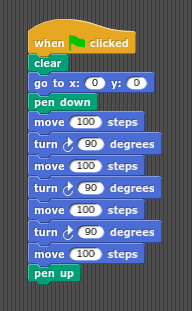
\includegraphics{basic_square.png}
\end{center}
Enter this and make sure it draws a square! One thing about this
program is that after it draws the square the arrow ends up pointing a
different direction to the direction it started in; can you fix this?
\begin{center}
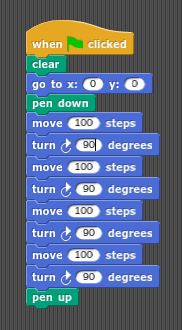
\includegraphics{basic_square_point.png}
\end{center}
Repeat
\begin{center}
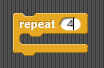
\includegraphics{repeat.png}
\end{center}
Can you use that to make the programme more succinct and readable? 
\begin{center}
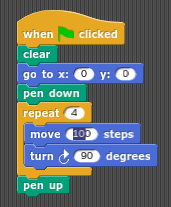
\includegraphics{repeat_square.png}
\end{center}


Now, look at this programme
\begin{center}
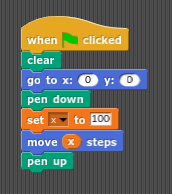
\includegraphics{variable.png}
\end{center}
Do the same to your square programme!
\begin{center}
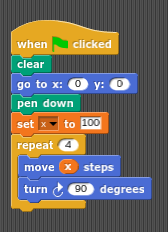
\includegraphics{variable_square.png}
\end{center}

\end{document}
